\section{Threshold Regime Analysis}\label{sec:theory_scaling}

\subsection{Entity Construction as MBR Decoding}\label{sec:mbr_theory}

Entity-level construction selects $\hat{y}_{\textup{MBR}} = \{e \in E_\cup : \hat{p}(e) > \alpha/(\alpha{+}1)\}$ under balanced set-overlap utility; $\alpha{=}1$ recovers majority vote (Proposition~\ref{prop:construction_mbr}; Table~\ref{tab:entity_construction}; Appendix~\ref{app:mbr_proof}).
Signal-derived weights $w_i$ yield quality-weighted MBR: $\hat{p}_w(e) = \sum_{i} w_i \, \mathbf{1}[e {\in} y_i] / \sum_{i} w_i$; weighting improves when $w_i$ correlates with instance quality but degrades otherwise (LP on SciERC: $\rho{\approx}0.2$; \S\ref{sec:prescriptive}), consistent with utility degradation on structured outputs \cite{eikema2025structured}.
We select $\varepsilon{=}0.05$ at the elbow of the compression curve, where LP-best selection advantage transitions from $+1.5$\,pp (compressed) to $+4.6$\,pp (non-compressed; Appendix~\ref{app:fewnerd_epsilon}).

\subsection{Scaling and Inverse Scaling}\label{sec:scaling}

Oracle F1 follows $F_1(N) = a - b \cdot N^{-c}$ ($R^2 > 0.999$; Figure~\ref{fig:oracle_scaling}): Few-NERD ($c{\approx}0.61$) scales comparably to reasoning tasks \cite{brown2024monkeys}, SciERC converges more slowly ($c{\approx}0.35$), yet confidence-based aggregation recovers ${<}1$\,pp---a persistent gap.
The gap persists across scales and families: scaling from 8B to 14B FT increases oracle headroom ($+1.2$\,pp) with minimal greedy gain ($+0.9$\,pp), and GPT-5.5 (200 Few-NERD instances, zero-shot) exhibits the same pattern---50\% degeneracy, SJ $\rho{=}0.346$, MV $+1.4$\,pp yet 6.8\,pp oracle headroom unrealized.\footnote{Of the 10.1\% of GPT-5.5 samples producing empty entity sets, 88\% correspond to gold-empty instances; true parse failures affect only 1.2\% of samples (19/1{,}600) and shift all reported metrics by ${<}0.5$\,pp. See Appendix~\ref{app:frontier_sc}.}
Degeneracy is model-family-dependent rather than scale-dependent (Qwen2.5: $31.7$--$46.2$\% vs.\ Qwen3: $13.0$\% vs.\ GPT-5.5: $50$\% on Few-NERD; Appendix~\ref{app:cross_scale}).

\begin{figure}[t]
\centering
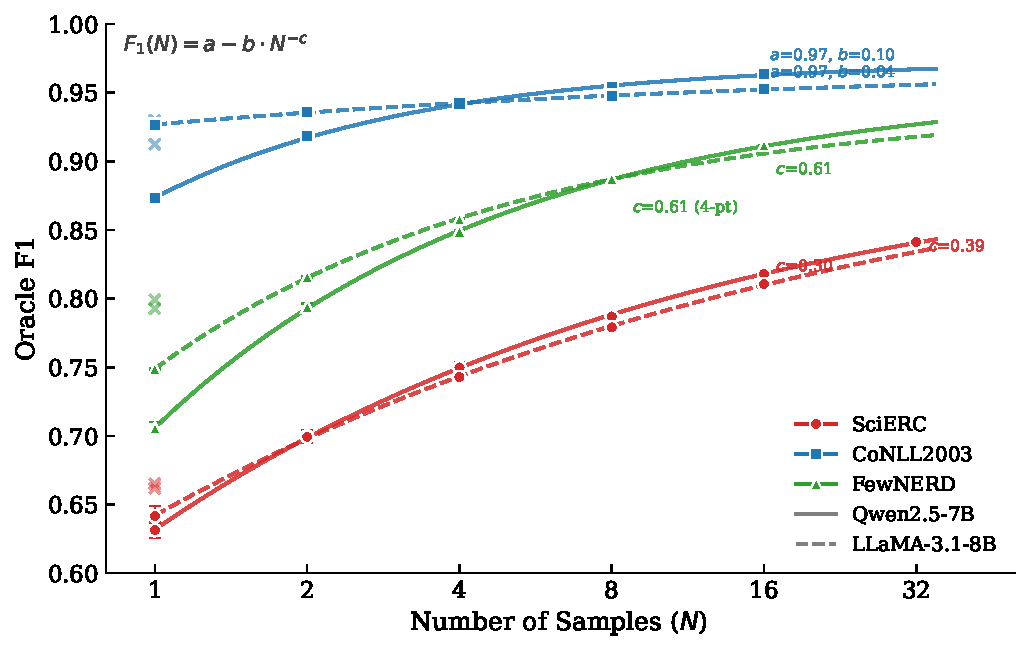
\includegraphics[width=\columnwidth]{figures/fig_oracle_scaling.pdf}
\caption{Oracle $F_1$ as a function of sample count $N$, fitted with $F_1(N) = a - b \cdot N^{-c}$. All fits $R^2 > 0.999$. Horizontal dashed lines: greedy ($T{=}0$) F1. The ceiling grows monotonically with $N$, but the correlation-selection gap (\S\ref{sec:selection_gap}) limits how much is actually recoverable.}
\label{fig:oracle_scaling}
\end{figure}

\paragraph{Inverse scaling under adaptive thresholds.}
Increasing $N$ \textit{decreases} construction F1 in 40 of 58 transitions ($p{<}0.05$; Appendix~\ref{app:n_scaling}).
Methods using $\theta{=}2/N$ are most affected ($-3.09$\,pp at $N{=}8$, $-6.90$\,pp at $N{=}16$ vs.\ greedy on Few-NERD); majority vote ($\theta{=}\tfrac{1}{2}$) reduces the delta to $-0.87$/$-0.60$\,pp---severity reduction, not immunity (Table~\ref{tab:theta_sweep}).
Inverse scaling concentrates in non-degenerate instances ($11.1$\% vs.\ $1.3$\% for degenerate; OR${=}0.109$; Appendix~\ref{app:degen_inverse}).
Few-shot demonstrations improve QE (CoNLL SJ $\rho$ $.30{\to}.44$) but not construction (all n.s.; Appendix~\ref{app:fs_error}).

\subsection{Degeneracy Decomposition}\label{sec:theory}

\noindent\textbf{Degeneracy Decomposition.}\label{thm:degeneracy_bound}
For any aggregation method $A$: $\mathbb{E}[\Delta F_1(A)] \leq (1 - D) \cdot G_{\textup{nd}}$,
where $D$ is the degeneracy rate and $G_{\textup{nd}}$ the oracle gap on non-degenerate instances.
For signal-based methods with alignment $\alpha \in [0,1]$, this tightens to $(1{-}D) \cdot G_{\textup{nd}} \cdot \alpha$ (proof in Appendix~\ref{app:bound_proof}).

\noindent The bound is an intentionally loose \textit{necessary condition test}: when $D{\to}1$ or $\alpha{\to}0$, no aggregation method can improve over greedy, regardless of implementation.
It identifies \textit{where} aggregation fails---screening for favorable conditions---rather than quantitatively predicting gains.
Across 16 configurations, all gains respect the bound; the low recovery ratio (3--12\%; Figure~\ref{fig:bound}) reflects its role as a screening test, not a tight estimate.
$\alpha$---not $D$---is the binding constraint ($\alpha{=}0.000$--$0.121$; $8$--$33{\times}$ tighter), and this conclusion is robust to signal combination (\S\ref{sec:robustness_main}), verifier-based construction (\S\ref{sec:verifier}), and $\theta_{\text{crit}} \in [0.60, 0.80]$.

\begin{figure}[t]
\centering

\includegraphics[width=\columnwidth]{fig_bound}
\caption{SC gain vs.\ degeneracy across 16 configurations (SciERC-specific $\alpha$). Red: signal-adjusted bound ($\alpha{=}0.068$); vertical dashed: $\theta_{\text{crit}}{=}0.70$; horizontal dotted: $\varepsilon{=}0.3$\,pp. All positive gains fall within the bound (right panel: ratio to weak bound, all ${<}0.13$).}
\label{fig:bound}
\end{figure}

\paragraph{Bound looseness.}
The decomposition is a necessary condition screen showing how degeneracy and alignment jointly suppress gains, not a quantitative prediction tool. Two sources of looseness dominate: (1)~the entity independence assumption---split-half correlation $r{=}0.395$--$0.578$ (Table~\ref{tab:fk_independence}) reveals substantial inter-entity correlation structure within instances, which the bound ignores; (2)~$\alpha$ is estimated conservatively as the minimum across instances rather than an instance-adaptive value, further widening the gap. Together these explain the 3--12\% recovery ratio (bound ratio $0.13$--$0.63$). The decomposition nonetheless identifies $\alpha{\to}0$, not degeneracy, as the binding constraint across all tested configurations.

MV improves F1 only if marginal-entity precision exceeds $F_1^{\textup{gr}}/2$ (Proposition~\ref{prop:entity_selection_bound}; Appendix~\ref{app:alpha_crit}).
Table~\ref{tab:alpha_crit} validates: at $N{=}8$, no dataset meets this condition ($\Delta$ from $-2.74$ to ${\approx}0$\,pp); CoNLL ($\alpha_{\textup{crit,eff}}{=}1.148 {>} 1$) makes MV gain structurally impossible.
